
\section{Results}
\label{sec:results}

We consider a large sensor network where the sensors can do relaying but the network itself is unreachable. To exfiltrate the data, an Unmanned Aerial Vehicle (UAV) flies by over the field. The UAV (running the MediaScope MSCloud \cite{mediascope}) carries the queries, gets the feature vectors from the sensors, and determines which sensed data to upload. In order to avoid detection and being power constrained, the UAV can only hang around for a very limited time. The UAV arbitrarily roams over the sensor network, and periodically extracts information from one of the sensors, however the network does not have any prior knowledge on its trace, and which node it will request the information.  Hence, from the network's perspective, the UAV can gather information from any of the nodes randomly. Without loss of generality, we assume the topology of the network is a mesh. For the unicast scenario, each node transmits its images to a destination node randomly. The QoI of the information extracted depends on timeliness and completeness if a top-K query was issued, and completeness if a spanner query was issued instead. 

We consider $W= 2 Mbps$, both unicast and flooding traffic, TDMA as the medium access control protocol, and an image size of 2 Mbytes.  In Figures \ref{fig:3dplot1} to \ref{fig:3dplot4}, we demonstrate network scalability as a function of QoI requirements for different traffic properties in a mesh setting.

\begin{figure}
\centering

    \subfigure[Unicast Traffic]{
        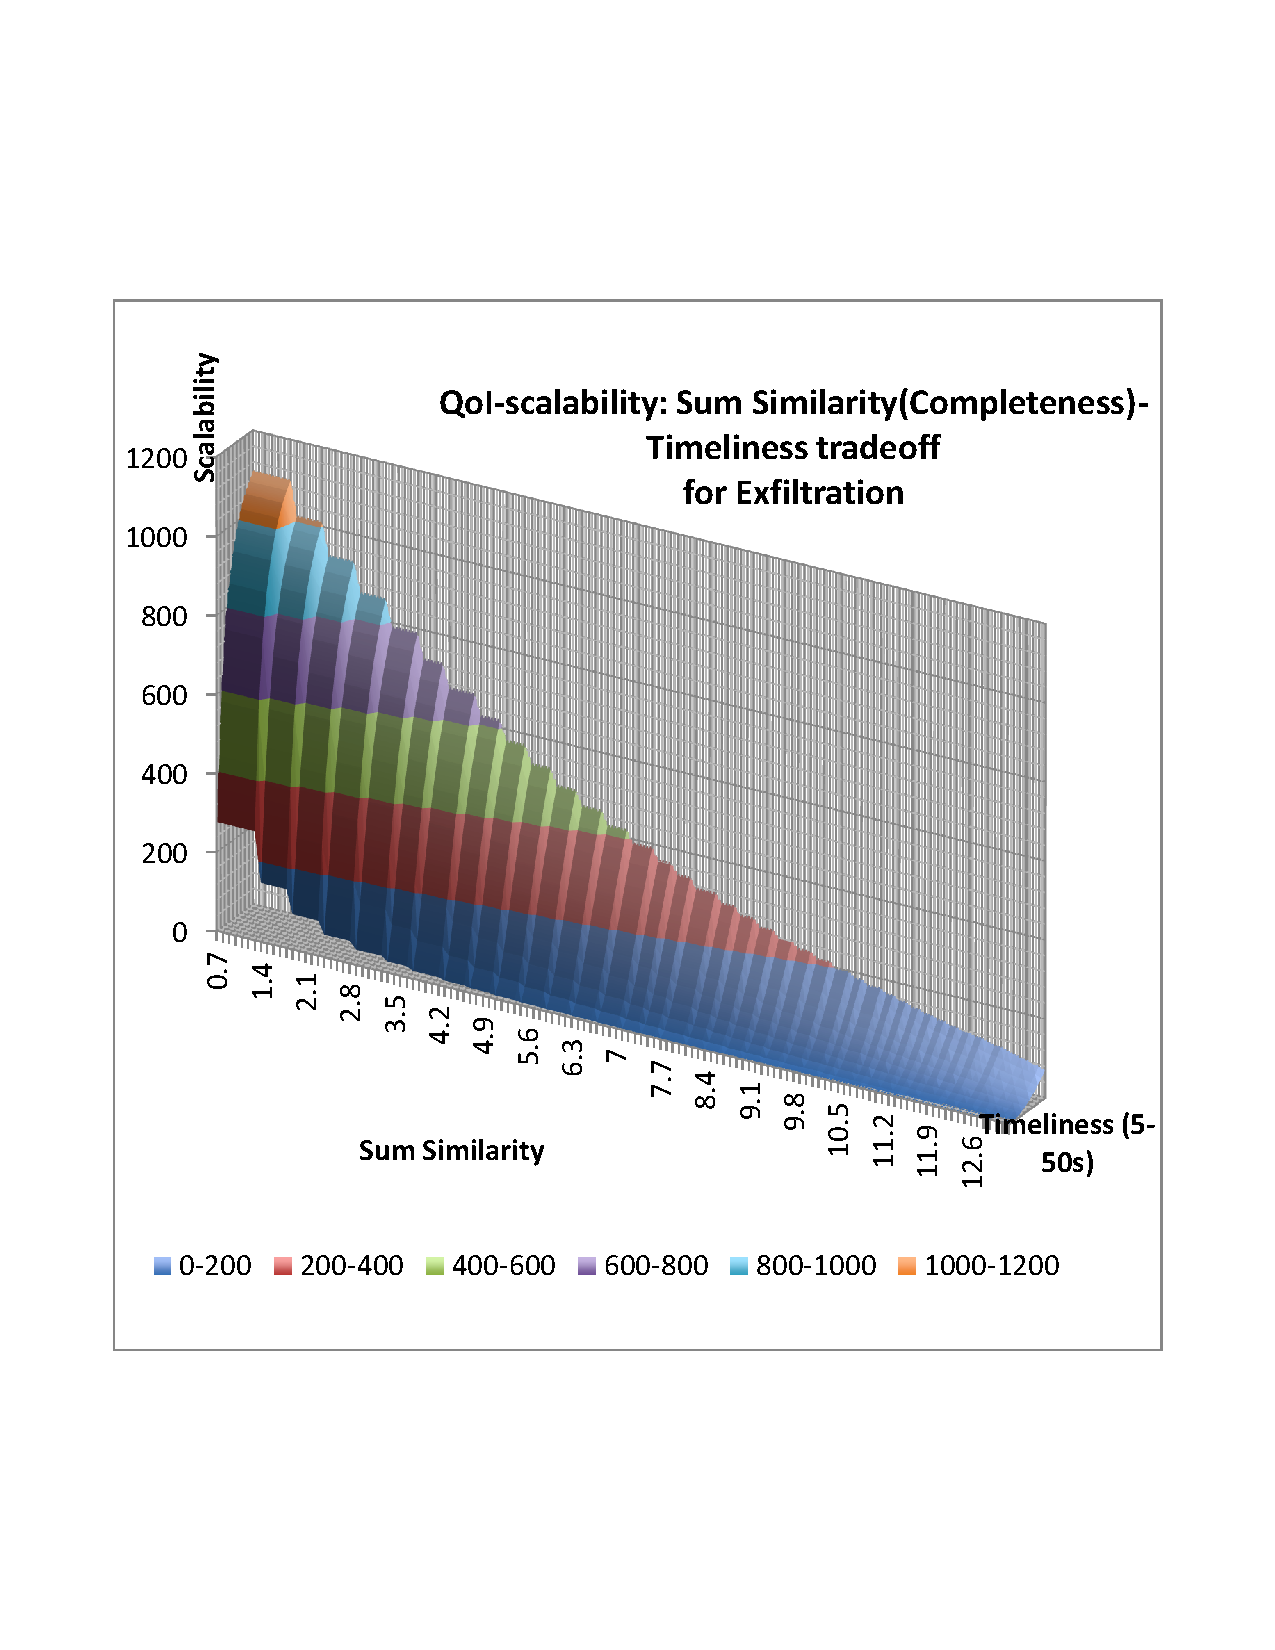
\includegraphics[scale=0.35]{figures/topk_uni.pdf}
        \label{fig:3dplot1}
        }

    \subfigure[Flooding]{
        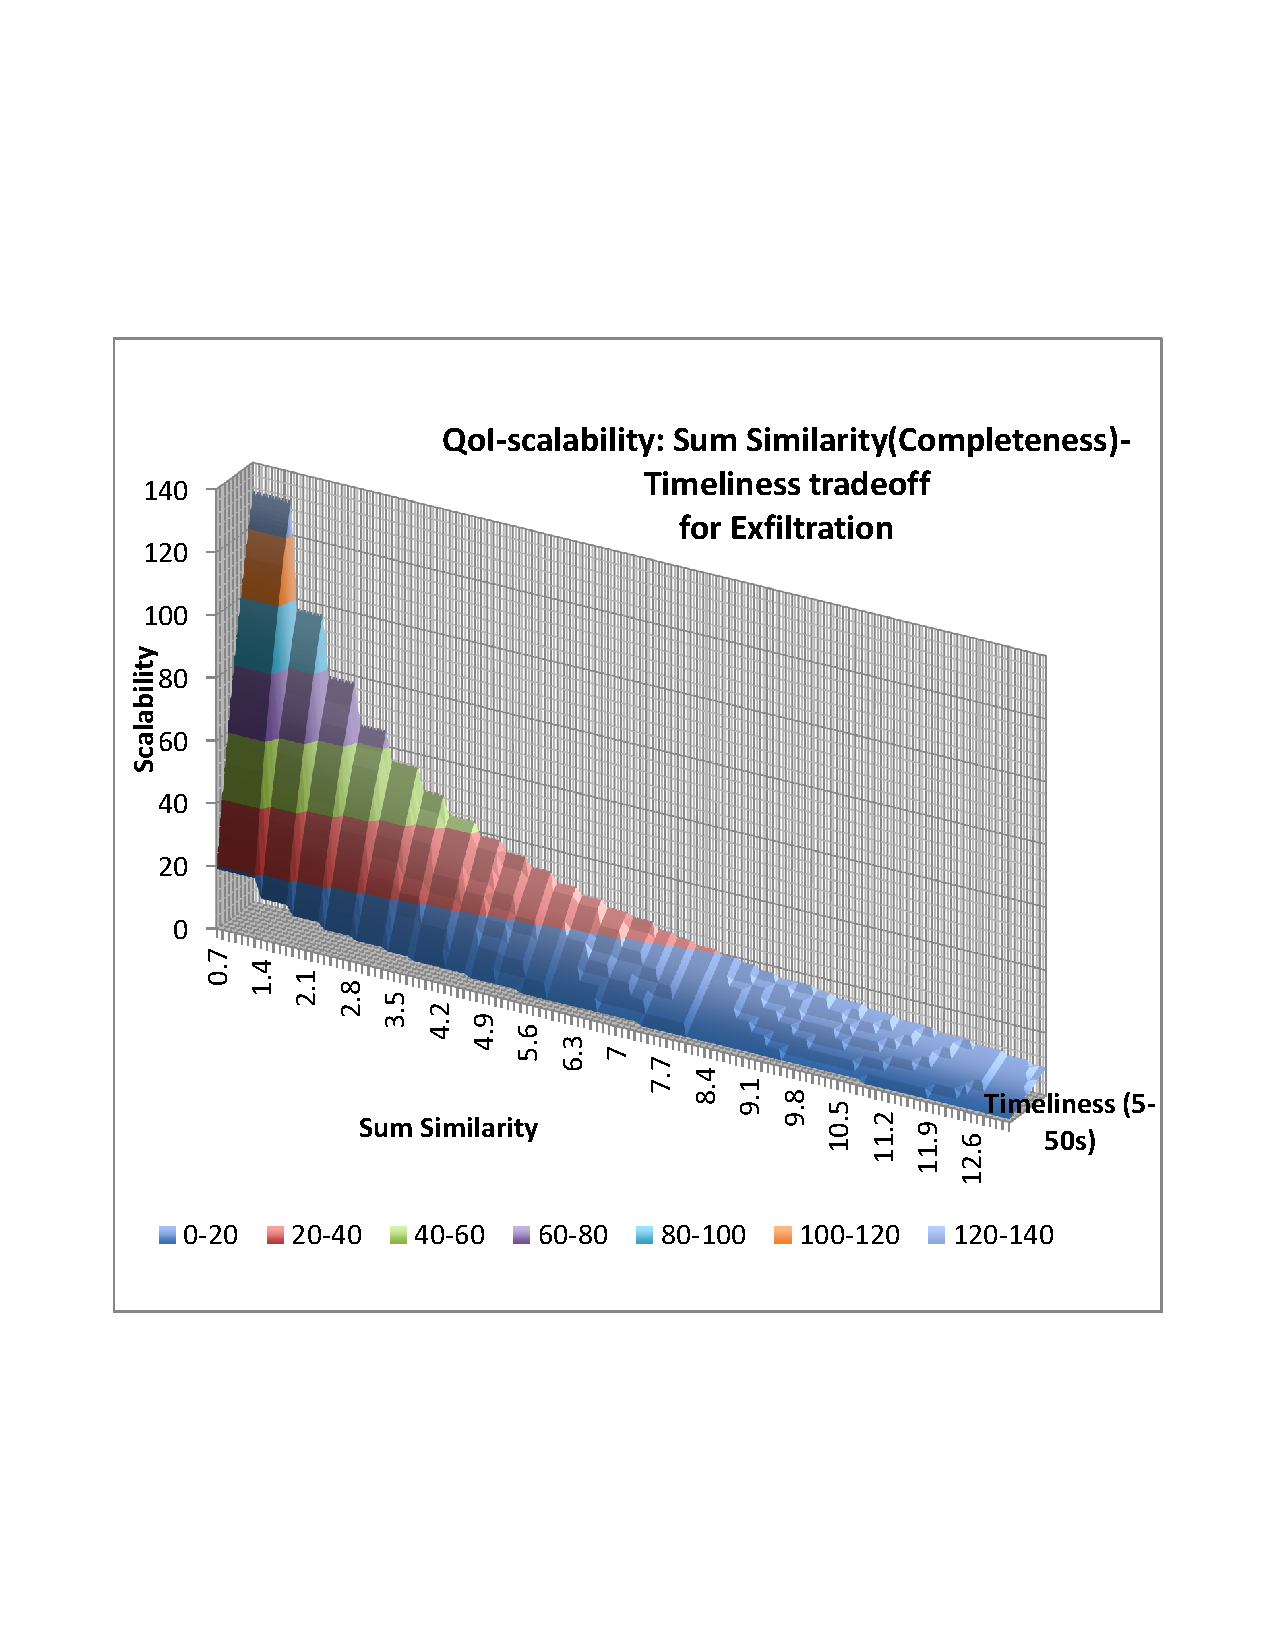
\includegraphics[scale=0.35]{figures/topk_fld.pdf}
        \label{fig:3dplot2}
        }

   \caption{Top-K:  Sum Similarity vs. Scalability vs. Timeliness}
\end{figure}


\begin{figure}
\centering
    \subfigure[Unicast Traffic]{
    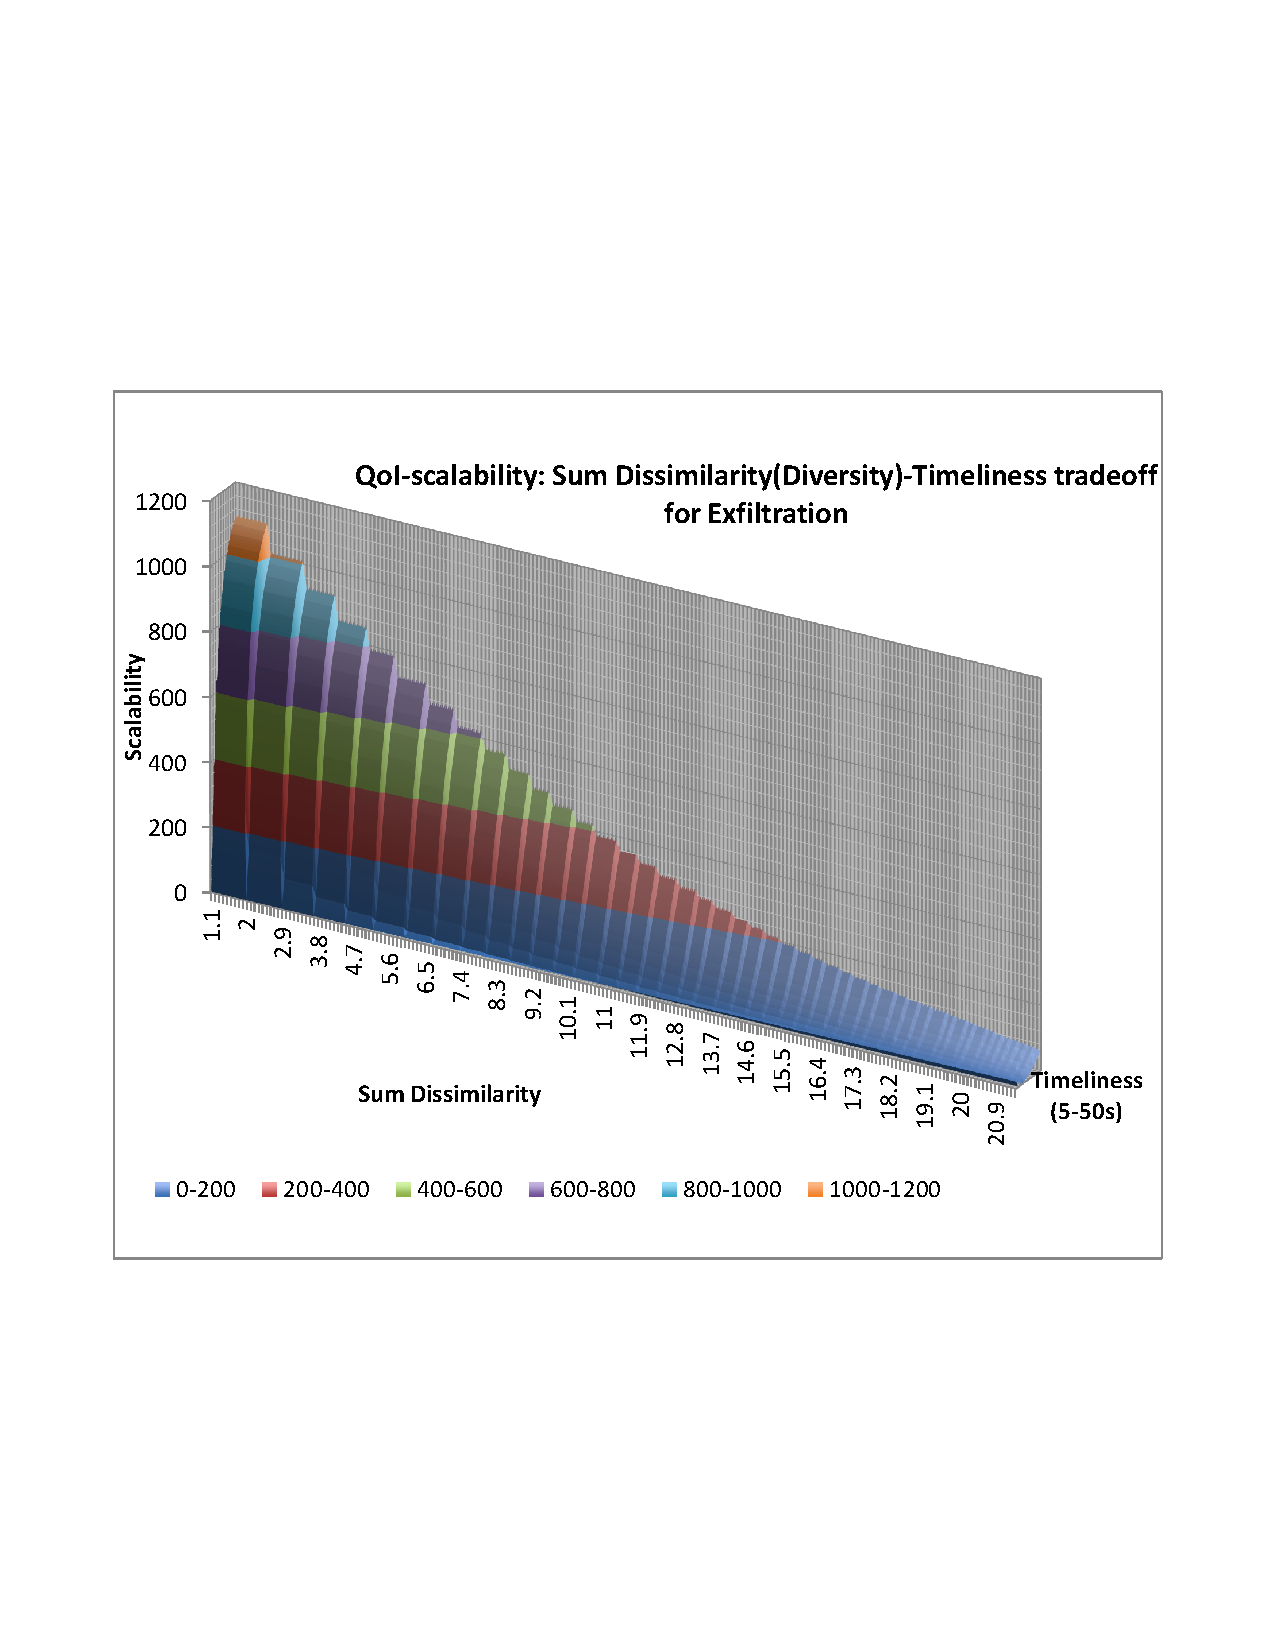
\includegraphics[scale=0.35]{figures/span_uni.pdf}
    \label{fig:3dplot3}
    }

    \subfigure[Flooding]{
    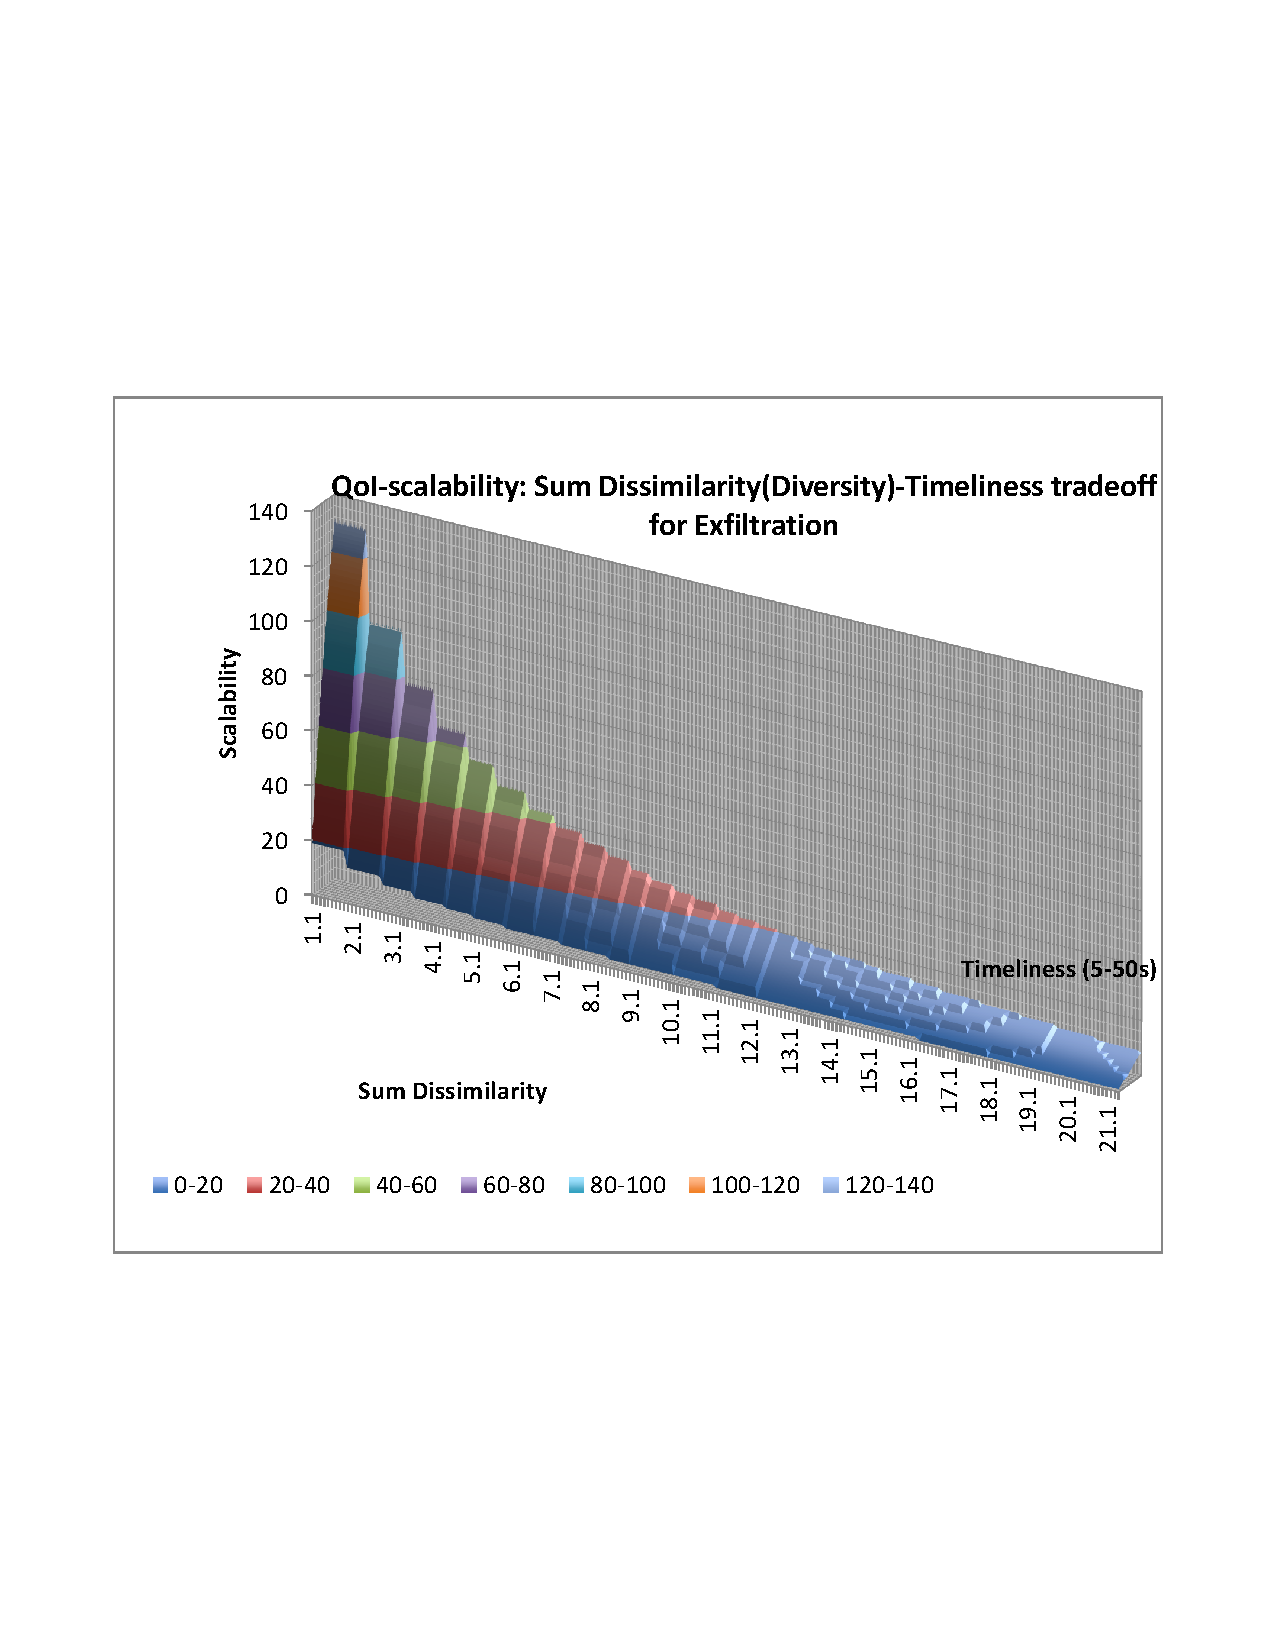
\includegraphics[scale=0.35]{figures/span_fld.pdf}
    \label{fig:3dplot4}
    }
   \caption{Spanner:  Sum Dissimilarity vs. Scalability vs. Timeliness}
\end{figure}

Clearly, there is a remarkable difference in the scalability depending upon the set QoI requirements.  The fact that QoI makes a difference is not surprising, but the {\em magnitude} of the impact is surprising, along with the fact that there are some critical thresholding points. Our preliminary work shows that scalability analysis with QoI awareness has the potential to open up new tradeoff points with significant potential benefits in scalability. For instance, it can potentially indicate when it makes sense to reduce QoI a bit and possibly gain significantly in scalability (e.g. from QoI=(10,5) to QoI=(10,10) in Figure \ref{fig:3dplot1}) and when such reductions will only give a marginal increase in scalability (e.g. from QoI=(3,40) to QoI=(3,45) in Figure \ref{fig:3dplot1}).

\subsection{Scalably Feasible QoI Regions}

Let us consider the special case where each node has at most one image. Note that even for such a setting, from fig. 4-5 the scalability of particularly flooding might be low. This leads to the following observation: To achieve a certain level of desired QoI \text{q}, which can be defined as $(C,T)$ for Top-K queries and $(D,T)$ for spanner queries, the completeness/diversity attribute necessitates a number $K_{req}(q)$ images to be collected. When each node can contribute with at most one picture, this implies a minimum network size of $K_{req}(q)$ that is necessary for the QoI level. On the other hand, the same QoI pair also results in a maximum network size $S(q)$ from the scalability framework.
When $S(q)<K_{req}(q)$, it is not possible to provide QoI level \text{q}. Hence, we state that the QoI level \text{q} is infeasible, or \emph{scalably infeasible}. 

This phenomenon defines the concept of \emph{scalably feasible QoI regions}, which define the set of QoI pairs that can be supported, given a given traffic structure. This region is given by a set of (completeness, timeliness) pairs for Top-K, and (diversity, timeliness) pairs for spanner queries. 
We demonstrate the scalably-feasible QoI regions in Figure \ref{fig:topkScalR}-{fig:spanScalR} for flooding traffic.

\begin{figure}
    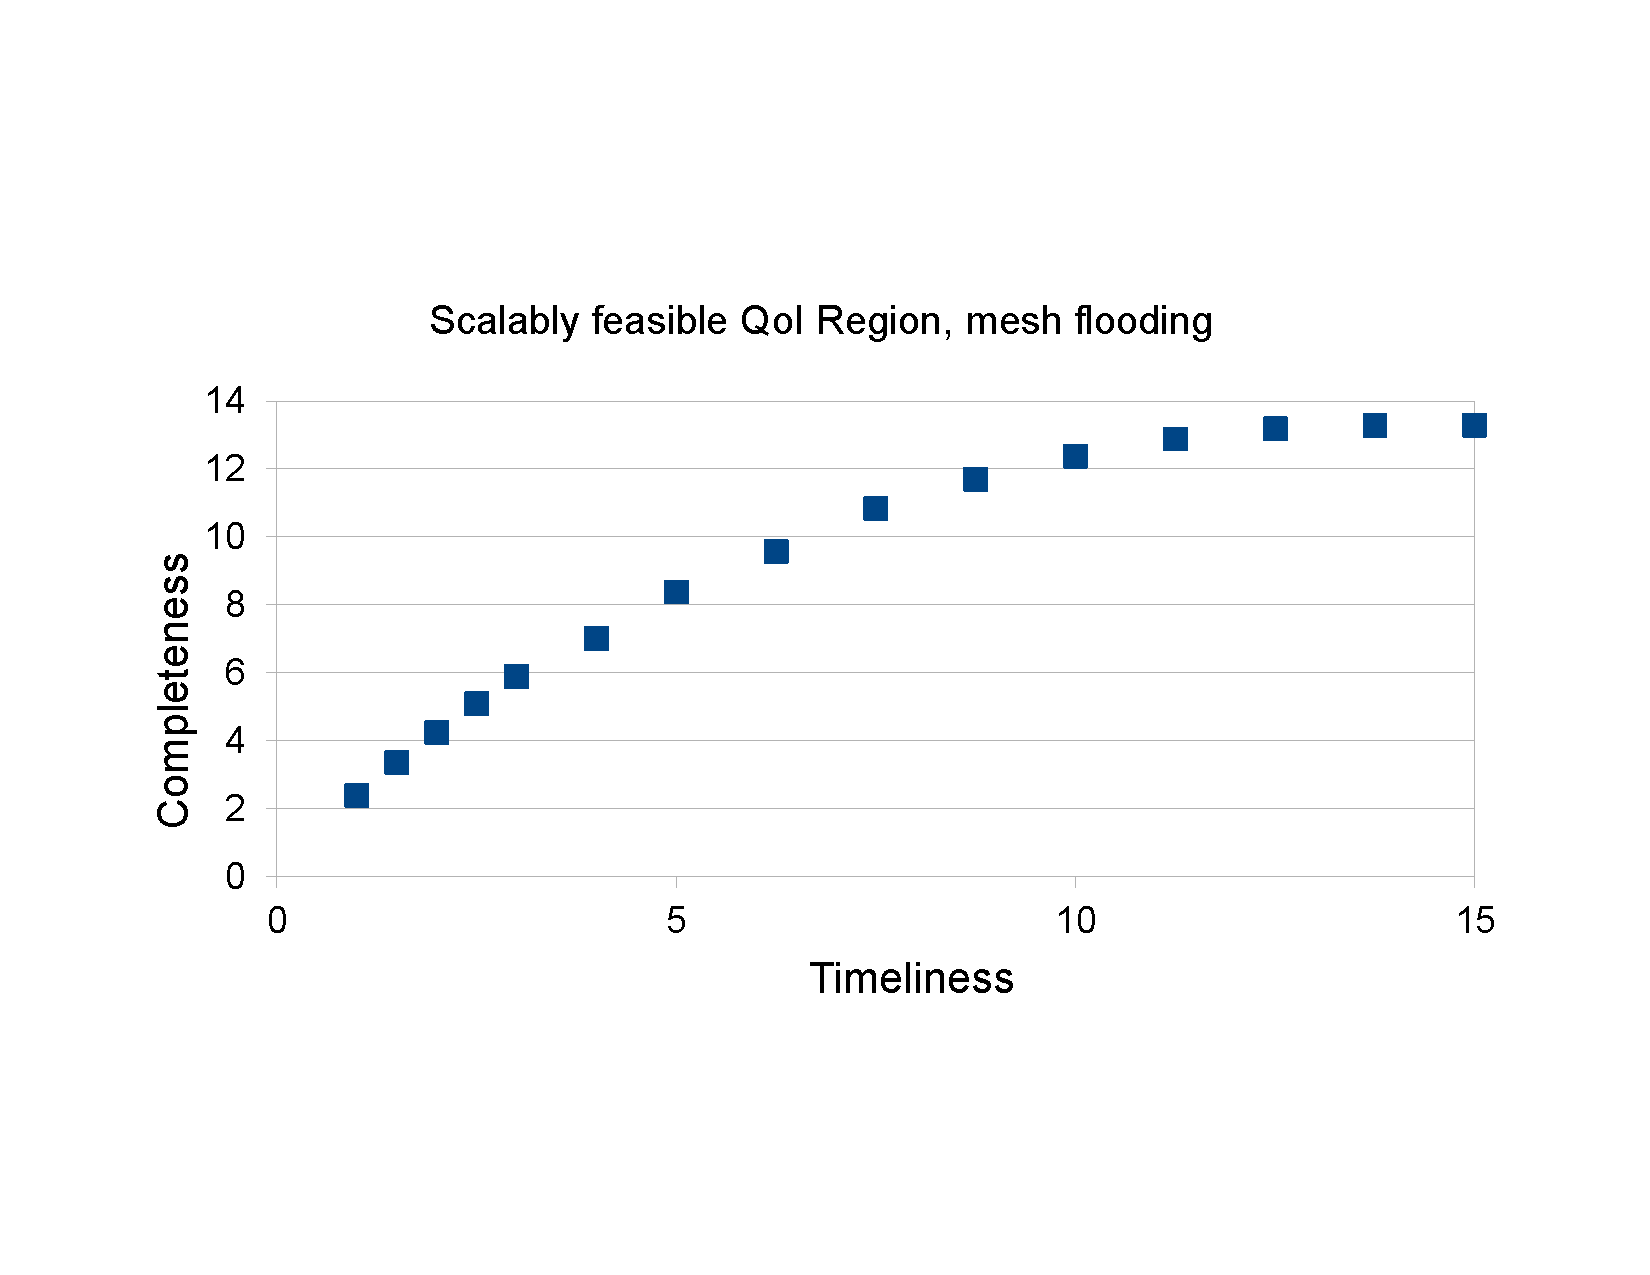
\includegraphics[scale=0.35]{figures/topkRegfld.pdf}
    \caption{Feasible Scalability Region of Spanner Algorithm, Flooding traffic}
    \label{fig:topkScalR}
\end{figure}


\begin{figure}
    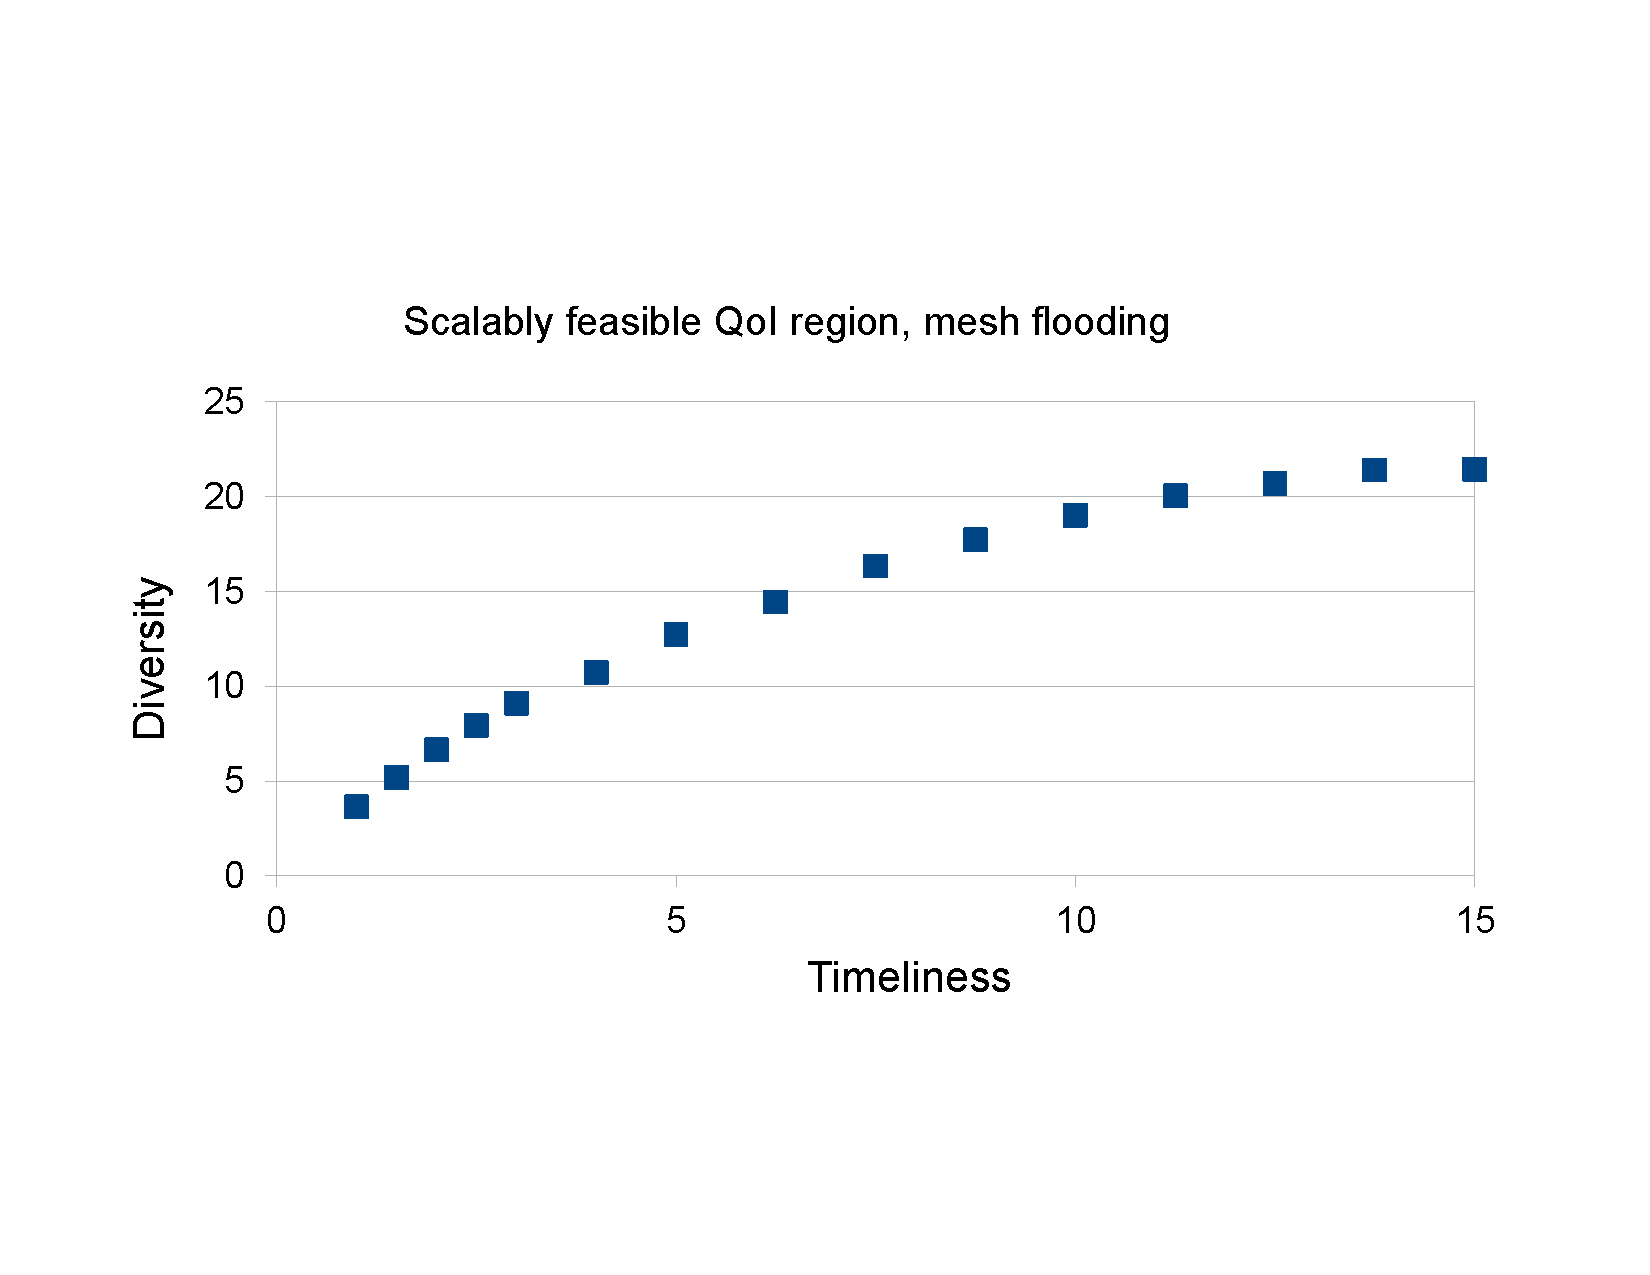
\includegraphics[scale=0.35]{figures/spanRegfld.pdf}
    \caption{Feasible Scalability Region of Spanner Algorithm, flooding traffic}
    \label{fig:spanScalR}
\end{figure}


While with the parameters in Fig. 4-5, no such problem is observed with unicast traffic unless timeliness is very low, for cases where the available bandwith is scarce, we have the scalability-wise feasability issue for unicast as well. We demonstrate results when the bandwidth is reduced to 500 Kbps for unicast in Figures \ref{fig:topkScalR}-\ref{fig:spanScalRuni}.

For both scenarios, these regions clearly
demonstrate the tradeoff between the completeness/diversity
that can be obtained and the timeliness that can be tolerated when system resources are scarce. 

\begin{figure}
    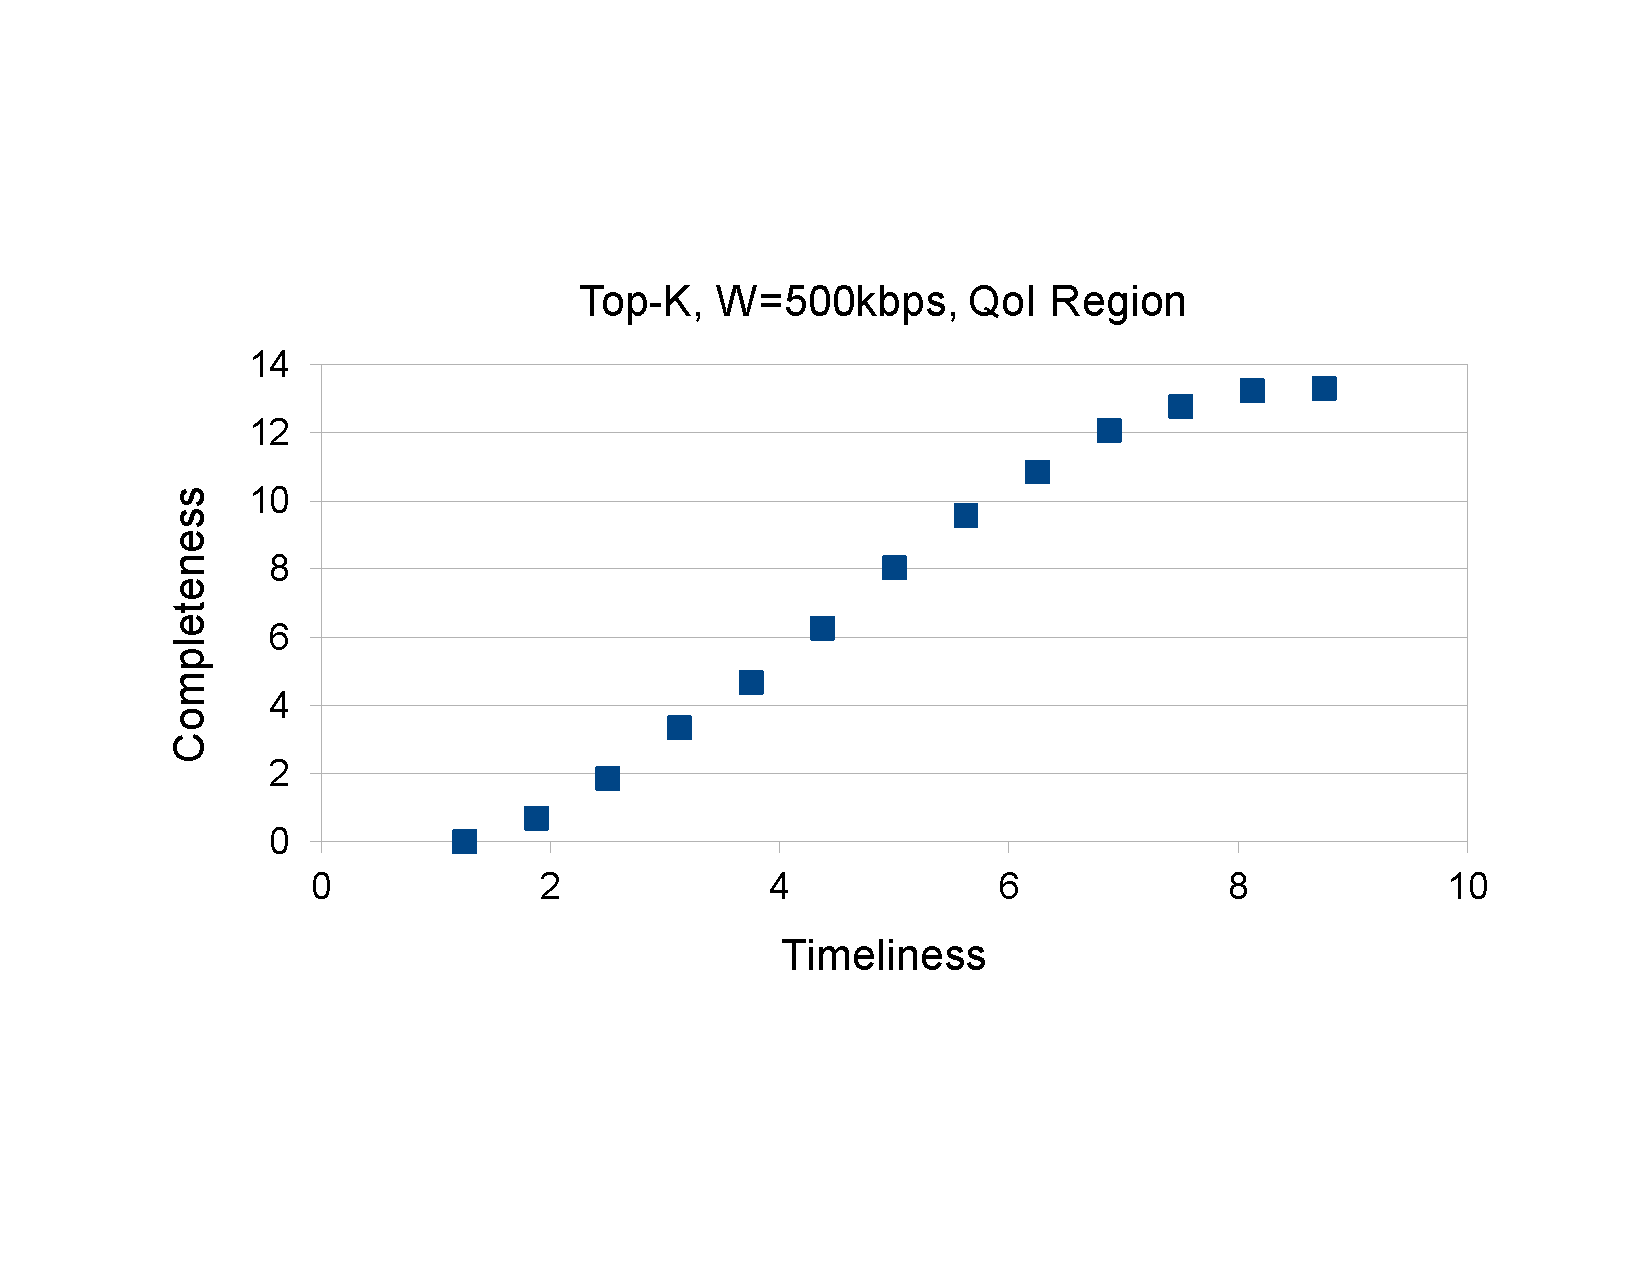
\includegraphics[scale=0.35]{figures/topkReg500kuni.pdf}
    \caption{Feasible Scalability Region of Top-K Algorithm, W=Unicast traffic, 500 Kbps}
    \label{fig:topkScalRuni}
\end{figure}

\begin{figure}
    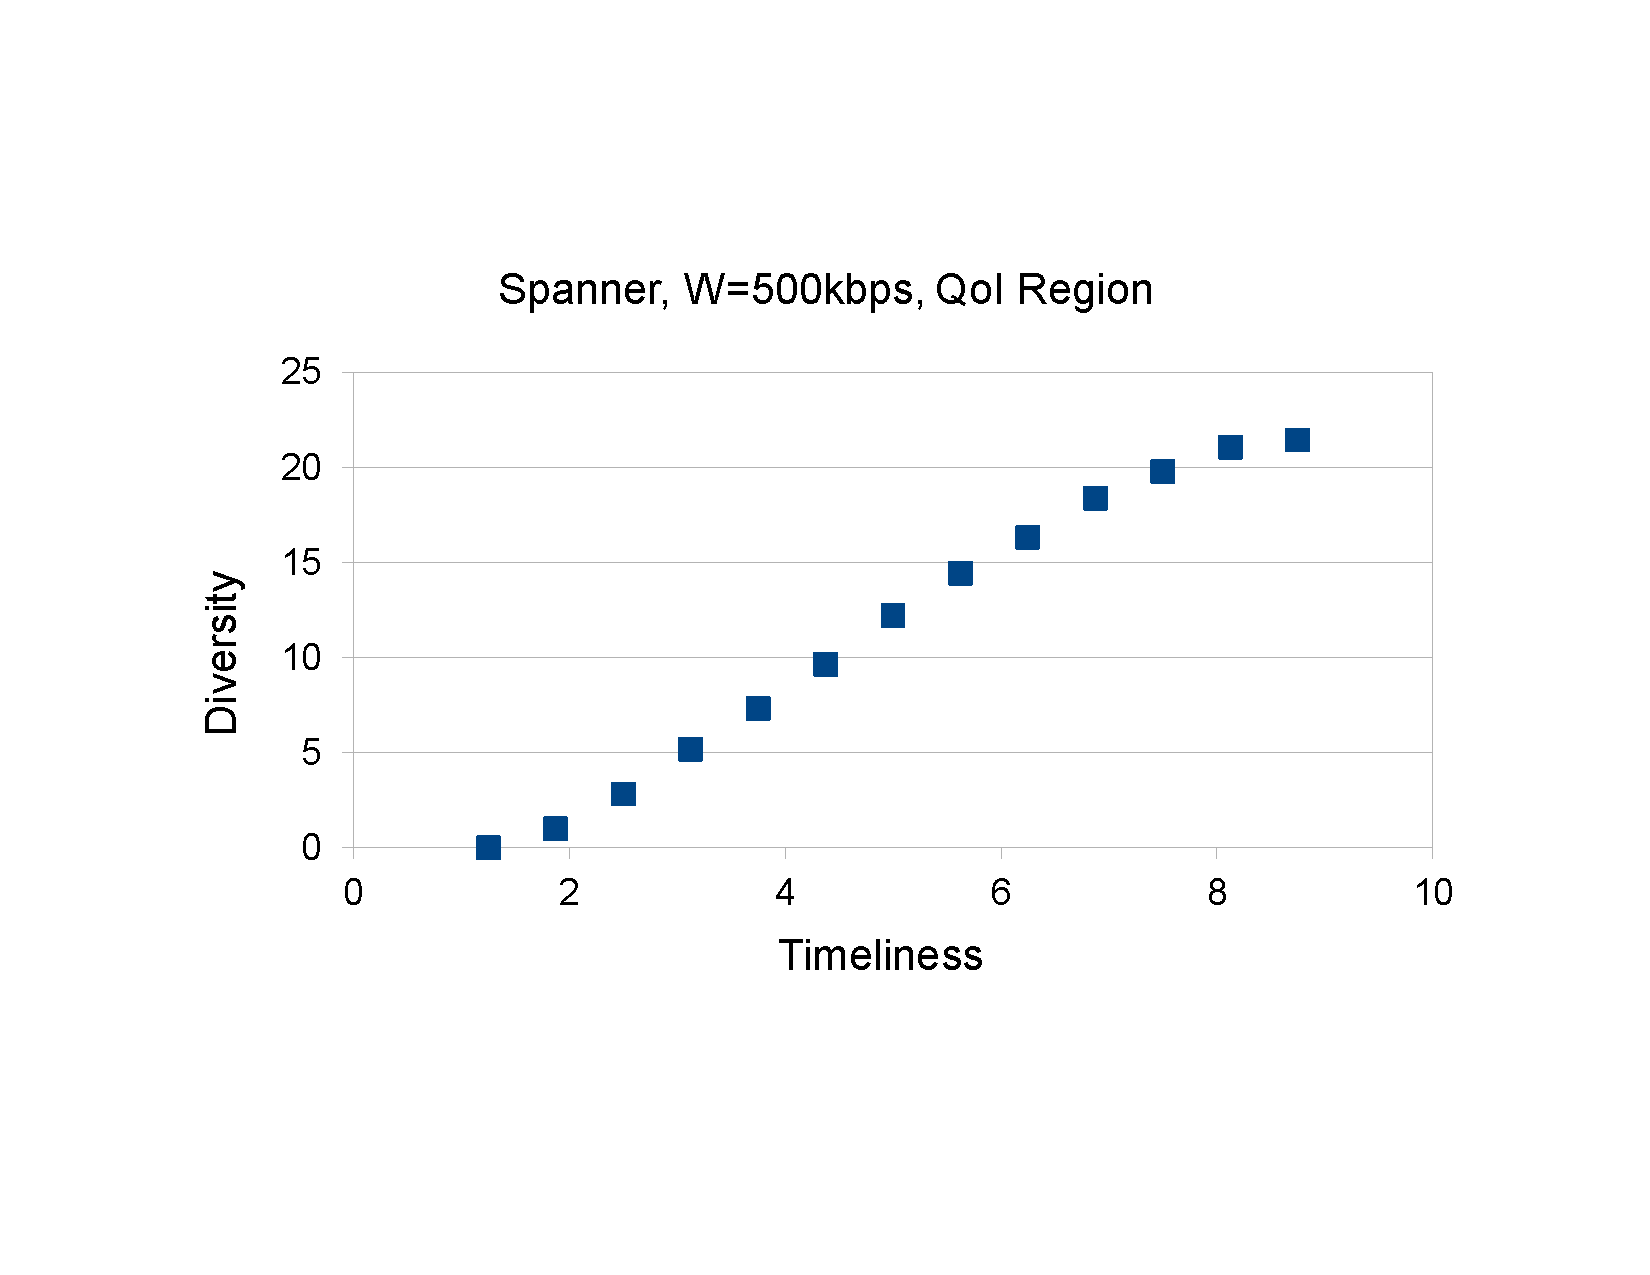
\includegraphics[scale=0.35]{figures/spanReg500k.pdf}
    \caption{Feasible Scalability Region of Spanner Algorithm, Unicast traffic, W=500 Kbps}
    \label{fig:spanScalRuni}
\end{figure}







